\section{Experimental Evaluation}
\label{sec:benchmarks}

The evaluation answers five questions.

\begin{description}
\item[Q1 (correctness).] Is state identity exact (two states identified if and only if they are
isomorphic) on every corpus workload, checked against an independent oracle?
(Table~\ref{tab:t1-exactness})
\item[Q2 (speed against the reference).] How does evolution time compare with the Wolfram
implementation of the same computation, and how does the ratio change with depth?
(Table~\ref{tab:t2-speedup}, Figure~\ref{fig:speedup})
\item[Q3 (parallel scaling).] How does evolution time change with the worker count, does that
depend on the rule, and what limits it? (Tables~\ref{tab:t8-scaling}, \ref{tab:t12-shapes},
\ref{tab:t13-memory}; Figure~\ref{fig:scaling})
\item[Q4 (device).] Where is the GPU faster than the CPU, and at what grid size does it saturate?
(Tables~\ref{tab:t7-gpu}, \ref{tab:t7b-gpu-corpus}, \ref{tab:t11-saturation})
\item[Q5 (attribution).] Which parts of the engine account for its speed, and does any of them
change the result? (Tables~\ref{tab:t9-ablation}, \ref{tab:t6-quotient}, \ref{tab:event-canon})
\end{description}

\subsection{Experimental Setup}

\begin{description}
\item[Hardware:] AMD EPYC 9174F (16 cores, 32 threads, one socket), 503\,GB RAM, NVIDIA RTX 4090 (24\,GB, compute capability 8.9), on bare metal. The cores are identical, so speedups divide comparable quantities. Workers are placed in the engine's default order, read from the cache topology at start-up: the cores of one last-level-cache domain and their SMT siblings are filled before the next domain is used. The Wolfram comparison of Table~\ref{tab:t2-speedup} needs a licensed Wolfram kernel and ran on a different machine, an Intel i9-14900K.
\item[Software:] Ubuntu 24.04, Linux 6.8, GCC with C++20, CUDA 12.0, Wolfram Language 14.3.
\item[Workloads:] A corpus of 17 workloads covering rule types (single and multiple rules; productive, idempotent, reductive and mixed-arity rules; several initial-state shapes), and deeper runs of the canonical Wolfram rule $\{\{x,y,z\}\} \to \{\{x,y,w\},\{y,z,w\}\}$ for the scaling and GPU measurements.
\item[Methodology:] Wall times are medians over repeated runs on an otherwise idle machine, and the two arms of any comparison are measured in the same session, because run-to-run variation on this machine exceeds many of the effects reported. Counts, instruction counts and \texttt{getrusage} figures are deterministic and come from a single run. The left-hand-side sweep of Figure~\ref{fig:lhs-scaling} reports the \emph{minimum} of its repeats, because interference from other load can only slow a run, and it starts a timed run only when the machine is idle.
\end{description}

\subsection{Correctness and Memory Footprint}
Every corpus workload is evolved single-threaded in the exact mode to the depth listed with it,
chosen so that the brute-force check stays tractable; depths differ between rows, so counts are
comparable within a column but not across rows. Its canonical state set, event set, causal
relation and branchial relation are compared with the reference implementation
(Table~\ref{tab:t1-exactness}), and each state set is checked against a brute-force isomorphism
oracle. All seventeen workloads agree exactly.

Table~\ref{tab:t3-deheap} gives the memory the same runs use. Arena bytes come from the arena's own
counter, which is deterministic, rather than from the resident set size. The global allocator is
called $455$ to $475$ times per run, for set-up that does not grow with the evolution, so calls
per event fall from $456$ on the smallest workload to $0.007$ on the largest.

\begin{table}[htbp]
\centering
\caption{Canonical states, events, causal edges and branchial edges for each corpus workload;
the brute-force oracle confirms every workload.}
\label{tab:t1-exactness}
% GENERATED by tools/dev/paper_tables.py -- do not edit.
% commit e6f5e5ef | Intel(R) Core(TM) i9-14900K, 20 GB RAM, Linux 5.15.167.4-microsoft-standard-WSL2 | source: tools/cost_matrix.cpp
%% arena bytes, all artifacts / neither relation: 286829596 / 179900636  (37.3% of the arena is the causal and branchial graphs)
\resizebox{\ifdim\width>\linewidth\linewidth\else\width\fi}{!}{%
\begin{tabular}{llrrrrrrrl}
\toprule
Workload & Class & Canon.\ states & Events & Causal & Branchial & Arena B & Heap B & Heap allocs & Exactness \\
\midrule
binary-growth & productive/arity2 & 874 & 36 & 873 & 872 & 0 & 1397512 & 3116132 & exact \\
wolfram-2to4 & productive/arity2 & 127 & 45 & 126 & 184 & 111 & 655024 & 1498684 & exact \\
triangle & productive/mixed-conn & 125 & 36 & 124 & 192 & 249 & 645784 & 1515100 & exact \\
reductive-2to1 & reductive/arity2 & 16 & 4 & 15 & 12 & 5 & 530968 & 1497212 & exact \\
idempotent-2to2 & idempotent/arity2 & 7 & 1 & 6 & 10 & 0 & 507920 & 1497164 & exact \\
self-loop & self-loop/arity2 & 2 & 2 & 1 & 0 & 0 & 363336 & 1251380 & exact \\
mixed-arity & mixed-arity & 7 & 7 & 6 & 5 & 0 & 440712 & 1513572 & exact \\
arity3-growth & arity3 & 154 & 65 & 153 & 152 & 0 & 542224 & 1498740 & exact \\
disconnected-lhs & disconnected & 127 & 1 & 126 & 248 & 63 & 634032 & 1497458 & exact \\
arity4-growth & arity4 & 34 & 23 & 33 & 32 & 0 & 460552 & 1497060 & exact \\
mixed-arity-lhs & mixed-arity/join & 2 & 2 & 1 & 0 & 0 & 380168 & 1251356 & exact \\
mixed-arity-init & mixed-arity/init & 5 & 4 & 4 & 0 & 0 & 398000 & 1513564 & exact \\
arity3-to-2 & arity-reductive & 5 & 4 & 4 & 0 & 0 & 398172 & 1513596 & exact \\
arity1-with-binary & arity1/mixed & 2 & 2 & 1 & 0 & 0 & 380152 & 1251340 & exact \\
cycle4-automorphic & automorphism & 68185 & 7 & 68184 & 109992 & 68184 & 179140120 & 201283020 & exact \\
star4-automorphic & automorphism & 68185 & 201 & 68184 & 56360 & 0 & 99249768 & 118459724 & exact \\
multi-rule & multi-rule & 238 & 36 & 237 & 214 & 108 & 705152 & 2060060 & exact \\
\bottomrule
\end{tabular}
}

\end{table}

\begin{table}[htbp]
\centering
\caption{Arena bytes, heap bytes, and global \texttt{operator new} calls during
evolution, per corpus workload, ordered by work performed.}
\label{tab:t3-deheap}
% GENERATED by tools/dev/paper_tables.py -- do not edit.
% commit e6f5e5ef | Intel(R) Core(TM) i9-14900K, 20 GB RAM, Linux 5.15.167.4-microsoft-standard-WSL2 | source: tools/cost_matrix.cpp
\resizebox{\ifdim\width>\linewidth\linewidth\else\width\fi}{!}{%
\begin{tabular}{lrrrrr}
\toprule
Workload & Canon.\ states & Events & Arena B & Heap allocs & Allocs per event \\
\midrule
idempotent-2to2 & 7 & 1 & 0 & 1497164 & 1497164.0000 \\
disconnected-lhs & 127 & 1 & 63 & 1497458 & 1497458.0000 \\
self-loop & 2 & 2 & 0 & 1251380 & 625690.0000 \\
mixed-arity-lhs & 2 & 2 & 0 & 1251356 & 625678.0000 \\
arity1-with-binary & 2 & 2 & 0 & 1251340 & 625670.0000 \\
reductive-2to1 & 16 & 4 & 5 & 1497212 & 374303.0000 \\
mixed-arity-init & 5 & 4 & 0 & 1513564 & 378391.0000 \\
arity3-to-2 & 5 & 4 & 0 & 1513596 & 378399.0000 \\
mixed-arity & 7 & 7 & 0 & 1513572 & 216224.5714 \\
cycle4-automorphic & 68185 & 7 & 68184 & 201283020 & 28754717.1429 \\
arity4-growth & 34 & 23 & 0 & 1497060 & 65089.5652 \\
binary-growth & 874 & 36 & 0 & 3116132 & 86559.2222 \\
triangle & 125 & 36 & 249 & 1515100 & 42086.1111 \\
multi-rule & 238 & 36 & 108 & 2060060 & 57223.8889 \\
wolfram-2to4 & 127 & 45 & 111 & 1498684 & 33304.0889 \\
arity3-growth & 154 & 65 & 0 & 1498740 & 23057.5385 \\
star4-automorphic & 68185 & 201 & 0 & 118459724 & 589351.8607 \\
\bottomrule
\end{tabular}
}

\end{table}

\begin{figure}[htbp]
\centering
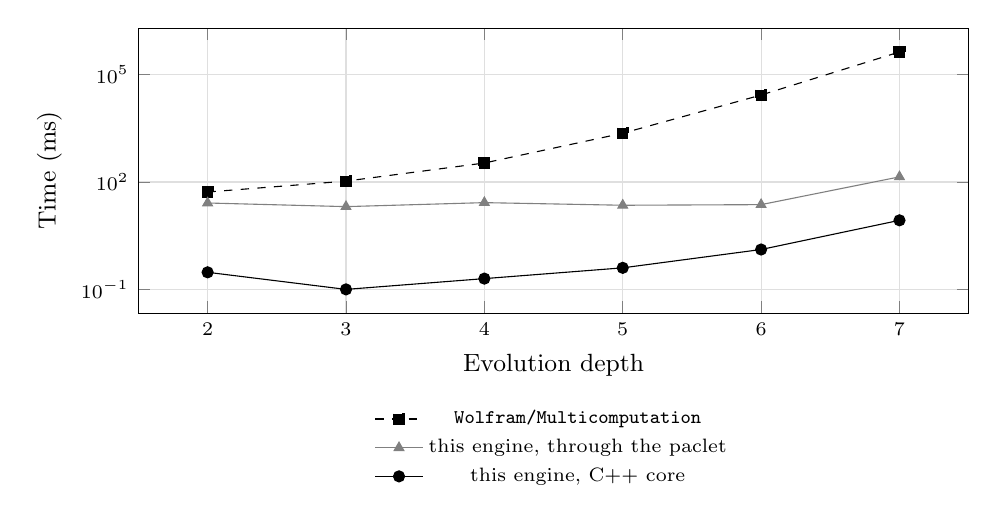
\begin{tikzpicture}
\begin{axis}[
    width=\linewidth, height=5.2cm,
    xlabel={Evolution depth}, ylabel={Time (ms)},
    ymode=log, xtick={2,3,4,5,6,7}, grid=major, grid style={gray!25},
    legend style={font=\scriptsize, at={(0.5,-0.30)}, anchor=north, legend columns=1,
                  draw=none, fill=none},
    label style={font=\small}, tick label style={font=\scriptsize},
]
% GENERATED by tools/dev/paper_tables.py -- do not edit.
% commit e6f26a9d | measured on Intel(R) Core(TM) i9-14900K, 31 GB RAM, Linux 5.15.167.4-microsoft-standard-WSL2 | load at start 0.19/0.23 (1m/15m) | source: reference/bench_authority.wls + tools/quotient_reconstruction_cost_probe.cpp (Wolfram kernel on cpu mask FFFF)
% paclet versions: HypergraphRewriting 1.0.0, SetReplace 0.3.196, Wolfram/Multicomputation 0.1.8

\addplot[mark=square*, black, dashed] coordinates {(2,52.5)(3,105.7)(4,339.1)(5,2298.6)(6,26830.7)(7,428264.0)};
\addlegendentry{\texttt{Wolfram/\allowbreak Multicomputation}}
\addplot[mark=triangle*, black!50] coordinates {(2,25.9)(3,20.5)(4,26.5)(5,22.4)(6,23.3)(7,139.0)};
\addlegendentry{this engine, through the paclet}
\addplot[mark=*, black] coordinates {(2,0.3)(3,0.1)(4,0.2)(5,0.4)(6,1.3)(7,8.5)};
\addlegendentry{this engine, C++ core}

\end{axis}
\end{tikzpicture}
\caption{Evolution time against depth for \texttt{MultiwaySystem}, the engine through the paclet,
and the engine's C++ core, on the same rule and initial state; all three give the same state and
causal-edge counts at every depth. The gap between the first and last series is the speedup of
Table~\ref{tab:t2-speedup}; the gap between the last two is the cost of the Wolfram interface.}
\label{fig:speedup}
\end{figure}

\subsection{Wall-Time Speedup}
The timed comparison is against the \texttt{Wolfram/\allowbreak Multicomputation} paclet's
\texttt{MultiwaySystem}, the published implementation of the same computation. The reference
implementation (Section~\ref{sec:background}) checks that all three agree on state and causal-edge
counts at every depth, and they do; its time is not reported. From depth four to seven the
engine's core is $\SpeedupAtLowDepth\times$ to $\SpeedupAtHighDepth\times$ faster than
\texttt{MultiwaySystem}, and the ratio increases with each depth. The depth-two time includes
\texttt{MultiwaySystem}'s one-time initialization, and at depths two to five the engine takes a
fraction of a millisecond, close to the timer's resolution, so the ratios at those depths are
lower bounds. At depth seven the engine takes $\CoreDeepMs$\,ms and
\texttt{MultiwaySystem} $\AuthorityDeepSeconds$\,s, both well above the resolution.

Each side is timed through its user-facing interface. Every \texttt{MultiwaySystem} property
returns a Wolfram \texttt{Graph} (\texttt{StatesGraph}, \texttt{CausalGraph},
\texttt{EvolutionGraph} and others), so its time includes building graphs. The engine is timed
twice: through its C++ API, and through the paclet, which serializes the request to the engine's
process over WXF, evolves, and builds the same kind of Wolfram structures on return. The difference
between the two is the cost of the Wolfram interface on the same computation: at depth
\SpeedupHighDepth{} it turns $\CoreDeepMs$\,ms into $\PacletDeepSeconds$\,s, a factor of
$\PacletOverheadDeep\times$. Through the paclet the engine is still $\PacletVsAuthorityDeep\times$
faster than \texttt{MultiwaySystem}.

\begin{table*}[htbp]
\centering
\caption{Wall time by depth against \texttt{MultiwaySystem} on
\texttt{wolfram-2to4}: $\{\{1,2\},\{2,3\}\} \to
\{\{1,2\},\{2,4\},\{4,3\}\}$ from $\{\{1,2\},\{2,3\}\}$. The engine is timed through its C++ API
and through the paclet (WXF and Wolfram structure construction included); the speedup column
divides \texttt{MultiwaySystem}'s time by the C++ core's. The reference implementation checks the
counts and is not timed.}
\label{tab:t2-speedup}
% GENERATED by tools/dev/paper_tables.py -- do not edit.
% commit e6f26a9d | measured on Intel(R) Core(TM) i9-14900K, 31 GB RAM, Linux 5.15.167.4-microsoft-standard-WSL2 | load at start 0.19/0.23 (1m/15m) | source: reference/bench_authority.wls + tools/quotient_reconstruction_cost_probe.cpp (Wolfram kernel on cpu mask FFFF)
% paclet versions: HypergraphRewriting 1.0.0, SetReplace 0.3.196, Wolfram/Multicomputation 0.1.8
{\footnotesize\setlength{\tabcolsep}{4pt}%
\resizebox{\ifdim\width>\linewidth\linewidth\else\width\fi}{!}{%
\begin{tabular}{rrrrrr}
\toprule
Depth & States & \texttt{MultiwaySystem} ms & Engine ms (paclet) & Engine ms (C++ core) & Speedup (core vs.\ \texttt{MultiwaySystem}) \\
\midrule
2 & 3 & 52.5 & 25.9 & 0.3 & 175$\times$ \\
3 & 4 & 105.7 & 20.5 & 0.1 & 1057$\times$ \\
4 & 5 & 339.1 & 26.5 & 0.2 & 1696$\times$ \\
5 & 6 & 2298.6 & 22.4 & 0.4 & 5746$\times$ \\
6 & 7 & 26830.7 & 23.3 & 1.3 & 20639$\times$ \\
7 & 8 & 428264.0 & 139.0 & 8.5 & 50384$\times$ \\
\bottomrule
\end{tabular}
}}

\end{table*}

\subsection{Quotient Exploration}
Quotient exploration expands each canonical state once, at its shallowest depth, so it produces far
fewer events than full expansion, and both give the same canonical state set
(Table~\ref{tab:t6-quotient}). At depth seven quotient exploration produces $28$ events where full
expansion produces $5{,}913$, and the reconstruction recovers all $5{,}913$, with their causal
edges and branchial pairs, from those $28$. The reconstruction's cost is below the resolution of
this measurement: at most depths the \texttt{quot.+recon} time is at or below the \texttt{quot.}
time, which is run-to-run variation on sub-millisecond timings.

\begin{table}[htbp]
\centering
\caption{Events and wall time, quotient exploration against full expansion, by depth on the
Wolfram rule; at every depth the reconstruction gives full expansion's event and causal counts
exactly.}
\label{tab:t6-quotient}
% GENERATED by tools/dev/paper_tables.py -- do not edit.
% commit 769b12ba | Intel(R) Core(TM) i9-14900K, 20 GB RAM, Linux 5.15.167.4-microsoft-standard-WSL2 | source: tools/quotient_reconstruction_cost_probe.cpp
\resizebox{\ifdim\width>\linewidth\linewidth\else\width\fi}{!}{%
\begin{tabular}{rrrrrrrrl}
\toprule
Depth & Events (full) & Causal (full) & ms (full) & Events (quot.) & ms (quot.) & Events (quot.+recon) & ms (quot.+recon) & Exact \\
\midrule
2 & 3 & 4 & 0.3 & 3 & 0.2 & 3 & 0.2 & exact \\
3 & 9 & 16 & 0.1 & 6 & 0.2 & 9 & 0.2 & exact \\
4 & 33 & 64 & 0.1 & 10 & 0.2 & 33 & 0.2 & exact \\
5 & 153 & 304 & 0.3 & 15 & 0.2 & 153 & 0.2 & exact \\
6 & 873 & 1744 & 1.6 & 21 & 0.4 & 873 & 0.4 & exact \\
7 & 5913 & 11824 & 16.0 & 28 & 1.7 & 5913 & 1.8 & exact \\
\bottomrule
\end{tabular}
}

\end{table}

\begin{figure}[htbp]
\centering
\begin{subfigure}{\linewidth}
\centering
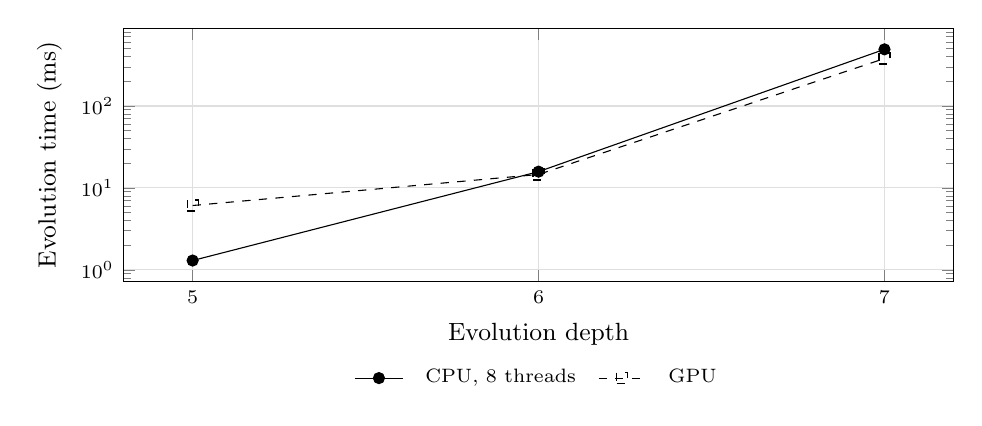
\begin{tikzpicture}
\begin{axis}[
    width=\linewidth, height=4.8cm,
    xlabel={Evolution depth}, ylabel={Evolution time (ms)},
    ymode=log, xtick={4,5,6,7,8,9}, grid=major, grid style={gray!25},
    legend style={font=\scriptsize, at={(0.5,-0.30)}, anchor=north, legend columns=2,
                  draw=none, fill=none, column sep=6pt},
    label style={font=\small}, tick label style={font=\scriptsize},
]
% GENERATED by tools/dev/paper_tables.py -- do not edit.
% commit 1d5bc1c9 | Intel(R) Core(TM) i9-14900K, 20 GB RAM, Linux 5.15.167.4-microsoft-standard-WSL2 | source: tools/bench_cpu_evolve.cpp + tools/bench_gpu_evolve.cpp

\addplot[mark=*, black] coordinates {(5,1.3)(6,15.8)(7,491.3)};
\addlegendentry{CPU, 8 threads}
\addplot[mark=square, black, dashed] coordinates {(5,6.1)(6,14.6)(7,379.9)};
\addlegendentry{GPU}

\end{axis}
\end{tikzpicture}
\caption{Evolution time against depth, the device against eight CPU threads
(Table~\ref{tab:t7-gpu}).}
\end{subfigure}

\vspace{2mm}
\begin{subfigure}{\linewidth}
\centering
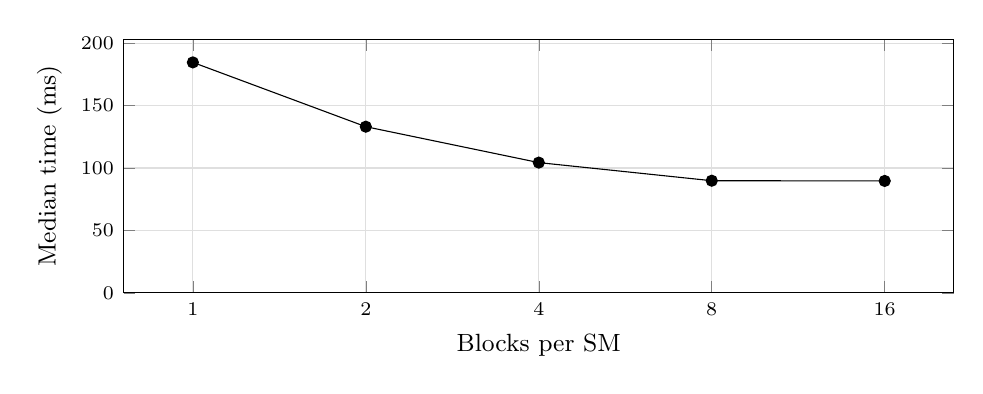
\begin{tikzpicture}
\begin{axis}[
    width=\linewidth, height=4.8cm,
    xlabel={Blocks per SM}, ylabel={Median time (ms)},
    xmode=log, log basis x=2, xtick={1,2,4,8,16}, xticklabels={1,2,4,8,16},
    ymin=0, grid=major, grid style={gray!25},
    label style={font=\small}, tick label style={font=\scriptsize},
]
% GENERATED by tools/dev/paper_tables.py -- do not edit.
% commit e264560 | measured on AMD EPYC 9174F 16-Core Processor, 503 GB RAM, Linux 6.8.0-138-generic | load at start 3.05/4.04 (1m/15m) | source: tools/bench_gpu_evolve.cpp (mode 2)

\addplot[mark=*, black] coordinates {(1,184.57)(2,133.06)(4,104.29)(8,89.78)(16,89.60)};

\end{axis}
\end{tikzpicture}
\caption{Median time against the resident kernel's grid size
(Table~\ref{tab:t11-saturation}).}
\end{subfigure}
\caption{Device comparison. The device is slower than eight CPU threads at depth five and faster
from depth six; time stops improving beyond eight blocks per streaming multiprocessor, the default
grid.}
\label{fig:gpu}
\end{figure}

\subsection{Device Comparison}
Both engines run the same rule, initial state, canonicalization mode and exploration strategy, and
report medians from one session (Figure~\ref{fig:gpu}, Table~\ref{tab:t7-gpu}). At depth five the
CPU is faster, because there is too little work to cover the device's fixed cost per evolution.
From depth six the device is faster than both CPU configurations, and the margin grows with depth,
to $\GpuSpeedupAtDeepest\times$ eight CPU threads at depth $\GpuDeepestDepth$ and more against one
thread.

Table~\ref{tab:t16-persistent} compares the resident kernel with a per-step \texttt{evolve()} on the
device, on the same workload. The resident kernel is $\PersistentSpeedupFour\times$ faster at depth
four, $\PersistentSpeedupFive\times$ at five, $\PersistentSpeedupSix\times$ at six and
$\PersistentSpeedupSeven\times$ at seven. The difference is a fixed cost per call:
\texttt{evolve()} takes $\PersistentEvolveConstLo$--$\PersistentEvolveConstHi$\,ms at depths four
to six while the state count grows from $\PersistentStatesLo$ to $\PersistentStatesHi$. From depth
\PersistentTieDepthWord{} ($\PersistentStatesTie$ states) the evolution outweighs that cost and the
two take the same time within run-to-run variation ($\PersistentSpeedupEight\times$ and
$\PersistentSpeedupNine\times$ at depths eight and nine).

\begin{table}[htbp]
\centering
\caption{End-to-end evolution time by depth on the Wolfram rule: GPU against CPU
at one and at eight threads.}
\label{tab:t7-gpu}
% GENERATED by tools/dev/paper_tables.py -- do not edit.
% commit 568b9fe | measured on AMD EPYC 9174F 16-Core Processor, 503 GB RAM, Linux 6.8.0-138-generic | load at start 0.16/0.93 (1m/15m) | source: tools/bench_cpu_evolve.cpp + tools/bench_gpu_evolve.cpp
{\footnotesize\setlength{\tabcolsep}{4pt}%
\resizebox{\ifdim\width>\linewidth\linewidth\else\width\fi}{!}{%
\begin{tabular}{rrrrrrrr}
\toprule
Steps & Raw states & Events & CPU 1t ms & CPU 8t ms & GPU ms & vs.\ CPU 1t & vs.\ CPU 8t \\
\midrule
5 & 401 & 400 & 4.1 & 2.6 & 3.8 & 1.09 & 0.70 \\
6 & 3867 & 3866 & 61.5 & 35.5 & 10.2 & 6.04 & 3.48 \\
7 & 45317 & 45316 & 3187.2 & 737.1 & 110.3 & 28.88 & 6.68 \\
\bottomrule
\end{tabular}
}}

\end{table}

\begin{table}[tb]
\centering
\caption{GPU against CPU across the corpus, one row per workload at its standard depth: the single
rules, the rule combinations, and the large symmetric states. Both engines run the same rules,
initial states, canonicalization mode and exploration strategy; medians share one session and one
iteration count.}
\label{tab:t7b-gpu-corpus}
% GENERATED by tools/dev/paper_tables.py -- do not edit.
% commit e264560 | measured on AMD EPYC 9174F 16-Core Processor, 503 GB RAM, Linux 6.8.0-138-generic | load at start 2.98/4.31 (1m/15m) | source: tools/bench_cpu_evolve.cpp + tools/bench_gpu_evolve.cpp
{\footnotesize\setlength{\tabcolsep}{4pt}%
\resizebox{\ifdim\width>\linewidth\linewidth\else\width\fi}{!}{%
\begin{tabular}{lrrrrrrr}
\toprule
Workload & Depth & Raw states & CPU 1t ms & CPU 16t ms & GPU ms & vs.\ CPU 1t & vs.\ CPU 16t \\
\midrule
wpp & 7 & 45317 & 549.9 & 175.0 & 89.8 & 6.13 & 1.95 \\
binary & 6 & 22 & 0.5 & 0.4 & 4.1 & 0.13 & 0.11 \\
wolfram24 & 6 & 9820 & 105.5 & 32.8 & 26.4 & 4.00 & 1.24 \\
triangle & 6 & 4 & 0.1 & 0.1 & 2.1 & 0.03 & 0.05 \\
arity3 & 6 & 7 & 0.1 & 0.2 & 3.6 & 0.02 & 0.05 \\
multirule & 6 & 49 & 46.0 & 26.4 & 106.0 & 0.43 & 0.25 \\
cycle4 & 6 & 40 & 24.4 & 11.2 & 78.5 & 0.31 & 0.14 \\
multiroot & 6 & 104 & 9.2 & 3.3 & 13.9 & 0.66 & 0.24 \\
disc2x2 & 6 & 1409 & 142.7 & 62.9 & 166.7 & 0.86 & 0.38 \\
growshrink3 & 5 & 8215 & 65.6 & 18.6 & 15.9 & 4.11 & 1.17 \\
wolftri & 6 & 10037 & 111.6 & 34.8 & 28.3 & 3.94 & 1.23 \\
arimix & 6 & 265 & 3.3 & 1.3 & 4.9 & 0.66 & 0.26 \\
allfour & 5 & 25571 & 227.2 & 67.8 & 37.3 & 6.09 & 1.82 \\
bigpath & 2 & 512 & 165.4 & 23.0 & 109.9 & 1.51 & 0.21 \\
bigcycle & 2 & 514 & 208.7 & 27.5 & 130.3 & 1.60 & 0.21 \\
bigstar & 2 & 34 & 1.5 & 1.3 & 12.0 & 0.12 & 0.11 \\
\bottomrule
\end{tabular}
}}

\end{table}

\begin{table}[htbp]
\centering
\caption{The resident kernel against a per-step \texttt{evolve()}, both on the
device, by depth on the same rule and initial state.}
\label{tab:t16-persistent}
% GENERATED by tools/dev/paper_tables.py -- do not edit.
% commit 18d1065d | measured on AMD EPYC 9174F 16-Core Processor, NVIDIA RTX 4090 | table generated on Intel(R) Core(TM) i9-14900K, 20 GB RAM, Linux 5.15.167.4-microsoft-standard-WSL2 | source: tools/bench_gpu_evolve.cpp (mode 0)
{\footnotesize\setlength{\tabcolsep}{4pt}%
\resizebox{\ifdim\width>\linewidth\linewidth\else\width\fi}{!}{%
\begin{tabular}{rrrrr}
\toprule
Depth & States & \texttt{evolve()} ms & Persistent ms & Speedup \\
\midrule
4 & 53 & 49.0 & 3.0 & $16.46\times$ \\
5 & 401 & 49.9 & 3.8 & $13.23\times$ \\
6 & 3,867 & 55.3 & 9.9 & $5.61\times$ \\
7 & 45,317 & 463.7 & 110.5 & $4.20\times$ \\
8 & 262,144 & 928.1 & 956.8 & $0.97\times$ \\
9 & 524,288 & 1716.2 & 1748.5 & $0.98\times$ \\
\bottomrule
\end{tabular}
}}

\end{table}

\subsection{Thread Scaling}
Strong scaling is measured on the Wolfram rule at depth seven, the deepest run in
Table~\ref{tab:t7-gpu}, at every power of two from one to thirty-two workers; the host has sixteen
cores, so workers beyond sixteen share a core with another worker through SMT. Wall time falls at
every step, by less each time, and by less again once the physical cores are used up, reaching a
speedup of $\MaxHostSpeedup\times$ at \MaxHostSpeedupThreads{} workers (Table~\ref{tab:t8-scaling}).
The expanded state set and the transition multiset are the same at every thread count and seed.
Table~\ref{tab:t12-shapes} gives the spread across rule shapes, and Table~\ref{tab:t13-memory} what
the extra time at high thread counts is spent on.

\begin{table}[htbp]
\centering
\caption{Strong scaling: median wall time and speedup over one worker by worker
count, Wolfram rule at depth seven ($28{,}542$ canonical and $45{,}317$ raw states at every
worker count), workers in the engine's default placement.}
\label{tab:t8-scaling}
% GENERATED by tools/dev/paper_tables.py -- do not edit.
% commit 1cbd805 | Intel(R) Core(TM) i9-14900K, 20 GB RAM, Linux 5.15.167.4-microsoft-standard-WSL2 | source: tools/bench_cpu_evolve.cpp

\begin{tabular}{rrrrrr}
\toprule
Threads & Steps & Canonical states & Raw states & Median ms & Speedup vs.\ 1 thread \\
\midrule
1 & 6 & 2677 & 3867 & 86.383 & 1.00 \\
4 & 6 & 2677 & 3867 & 25.152 & 3.43 \\
8 & 6 & 2677 & 3867 & 15.258 & 5.66 \\
\bottomrule
\end{tabular}

\end{table}

\begin{figure}[htbp]
\centering
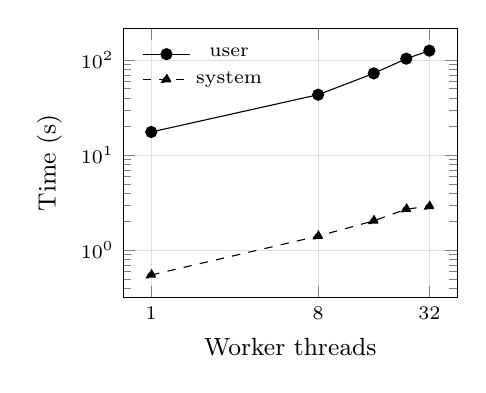
\begin{tikzpicture}
\begin{axis}[
    width=0.48\textwidth, height=5.0cm,
    xlabel={Worker threads}, ylabel={Time (s)},
    xmode=log, log basis x=2, xtick={1,8,32}, xticklabels={1,8,32},
    ymode=log, grid=major, grid style={gray!25},
    legend style={font=\scriptsize, at={(0.03,0.97)}, anchor=north west, draw=none, fill=none},
    label style={font=\small}, tick label style={font=\scriptsize},
]
% GENERATED by tools/dev/paper_tables.py -- do not edit.
% commit ca4a52b | measured on AMD EPYC 9174F 16-Core Processor, 503 GB RAM, Linux 6.8.0-138-generic | load at start 2.62/3.47 (1m/15m) | source: tools/sampling_cost_smoke.cpp under procstat.measure

\addplot[mark=*, black] coordinates {(1,17.55)(8,43.28)(16,72.58)(24,103.58)(32,125.83)};
\addlegendentry{user}
\addplot[mark=triangle*, black, dashed] coordinates {(1,0.55)(8,1.41)(16,2.04)(24,2.71)(32,2.90)};
\addlegendentry{system}

\end{axis}
\end{tikzpicture}
\caption{User and system time against worker count, for the runs of
Table~\ref{tab:t13-memory}: across a $\ThreadSweepFactor\times$ increase in workers, user time
grows $\UserTimeGrowth\times$ and system time, thirty to forty-five times smaller, grows
$\SysTimeGrowth\times$.}
\label{fig:scaling}
\end{figure}

\subsection{Parallel Efficiency by Rule Shape}
The amount of parallel work in a run depends on the rule. Table~\ref{tab:t12-shapes} measures two
rules at every thread count: a one-edge left-hand side, which matches by an index scan and expands
each state narrowly, and a two-edge left-hand side, which matches by a join and produces a wider
frontier. With both sized to seconds of single-threaded work, their efficiencies are within a few
points of each other at every thread count (the lower of the two is $\EffAtEight$ at eight threads
and $\EffAtSixteen$ at sixteen), and both still gain in wall time at thirty-two threads. The
decline is not thread start-up, since both single-threaded runs take seconds; it starts at the
thread count that first uses a second L3 domain (Section~\ref{sec:memory-scaling}).
Section~\ref{sec:lhs-space} measures the same size axis at four sizes and greater depths, together
with two other properties of the left-hand side.

\begin{table}[htbp]
\centering
\caption{Wall time and parallel efficiency by thread count for a one-edge and a
two-edge left-hand side.}
\label{tab:t12-shapes}
% GENERATED by tools/dev/paper_tables.py -- do not edit.
% commit e264560 | measured on AMD EPYC 9174F 16-Core Processor, 503 GB RAM, Linux 6.8.0-138-generic | load at start 3.05/4.04 (1m/15m) | source: tools/sampling_cost_smoke.cpp
{\footnotesize\setlength{\tabcolsep}{4pt}%
\resizebox{\ifdim\width>\linewidth\linewidth\else\width\fi}{!}{%
\begin{tabular}{rrrrr}
\toprule
Threads & \multicolumn{2}{c}{one-edge LHS} & \multicolumn{2}{c}{two-edge LHS} \\
 & ms & eff. & ms & eff. \\
\midrule
1 & 18076.0 & 1.00 & 12228.5 & 1.00 \\
2 & 9779.1 & 0.92 & 6746.5 & 0.91 \\
4 & 7034.7 & 0.64 & 4816.4 & 0.63 \\
8 & 5561.6 & 0.41 & 4156.2 & 0.37 \\
16 & 4606.0 & 0.25 & 3612.3 & 0.21 \\
24 & 4414.6 & 0.17 & 3522.3 & 0.14 \\
32 & 4097.0 & 0.14 & 3291.2 & 0.12 \\
\bottomrule
\end{tabular}
}}

\end{table}

\subsection{Left-Hand-Side Properties}
\label{sec:lhs-space}

A left-hand side has three independent properties, each of which changes the matching problem:

\begin{itemize}
\item \textbf{Size}: the number of edges to bind. Each edge adds a factor to the search and a
      constraint that prunes it.
\item \textbf{Arity}: the number of vertices per edge, which sets how much of the state one bound
      edge determines.
\item \textbf{Connectivity}: how the edges share vertices. A path shares one vertex between
      consecutive edges; a star shares one vertex among all of them; a ring has no end; and a
      left-hand side with components that share no vertex is matched as a cartesian product,
      quadratic in the state size for two components.
\end{itemize}

Figure~\ref{fig:time-corpus} gives the wall times of the sweep's ten timed workloads at every thread
count, each at the deepest depth whose single-threaded run fits the sweep's time budget, and
Figure~\ref{fig:lhs-scaling} gives the same measurements as parallel efficiency along each
property. Every curve in Figure~\ref{fig:time-corpus} falls through 32 threads, mostly below
sixteen: going from one thread to eight divides wall time by $2.3$ (the star) to $4.5$ (the
mixed-arity chain), and going from sixteen threads to 32 reduces it by a further $4.6$ to $23.7$
percent.

\begin{figure}[htbp]
\centering
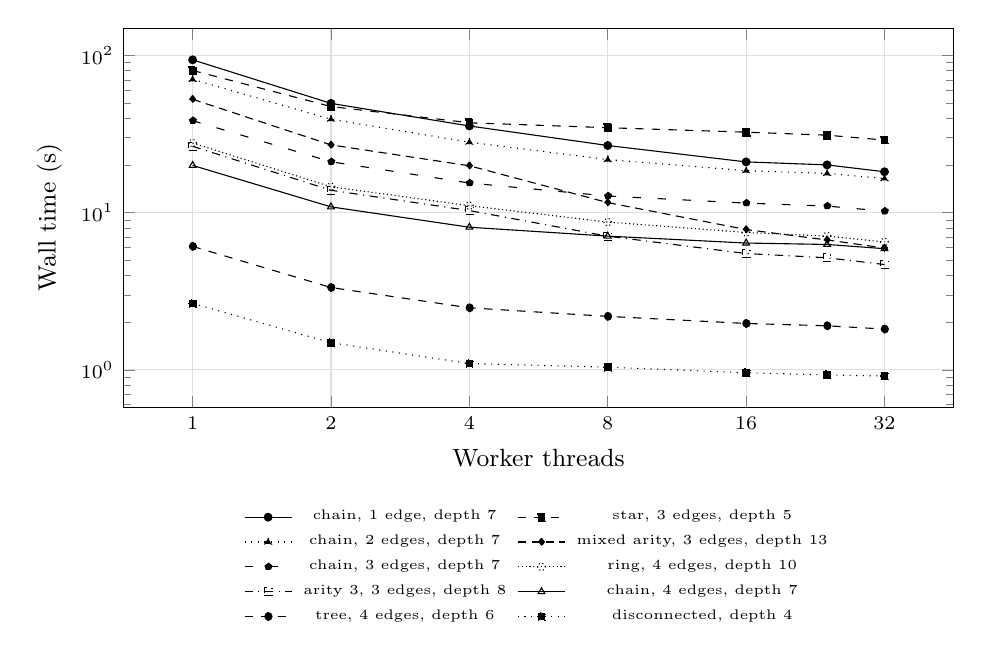
\begin{tikzpicture}
\begin{axis}[
    width=\linewidth, height=6.4cm,
    xlabel={Worker threads}, ylabel={Wall time (s)},
    xmode=log, log basis x=2, xtick={1,2,4,8,16,32}, xticklabels={1,2,4,8,16,32},
    ymode=log, grid=major, grid style={gray!25},
    legend style={font=\tiny, at={(0.5,-0.24)}, anchor=north, legend columns=2,
                  draw=none, fill=none, column sep=2pt, inner xsep=1pt},
    label style={font=\small}, tick label style={font=\scriptsize},
]
% GENERATED by tools/dev/paper_tables.py -- do not edit.
% commit 0ada228c | measured on AMD EPYC 9174F 16-Core Processor | table generated on Intel(R) Core(TM) i9-14900K, 31 GB RAM, Linux 5.15.167.4-microsoft-standard-WSL2 | source: tools/dev/rich_sweep.sh over tools/sampling_cost_smoke.cpp

\addplot[mark=*, black, solid, mark size=1.4pt] coordinates {(1,93.878)(2,49.606)(4,35.632)(8,26.764)(16,21.049)(24,20.145)(32,18.221)};
\addlegendentry{chain, 1 edge, depth 7}
\addplot[mark=square*, black, dashed, mark size=1.4pt] coordinates {(1,80.373)(2,47.377)(4,37.334)(8,34.735)(16,32.536)(24,31.135)(32,28.995)};
\addlegendentry{star, 3 edges, depth 5}
\addplot[mark=triangle*, black, dotted, mark size=1.4pt] coordinates {(1,70.547)(2,39.330)(4,28.093)(8,21.781)(16,18.513)(24,17.780)(32,16.494)};
\addlegendentry{chain, 2 edges, depth 7}
\addplot[mark=diamond*, black, densely dashed, mark size=1.4pt] coordinates {(1,52.686)(2,27.002)(4,19.892)(8,11.596)(16,7.813)(24,6.708)(32,5.962)};
\addlegendentry{mixed arity, 3 edges, depth 13}
\addplot[mark=pentagon*, black, loosely dashed, mark size=1.4pt] coordinates {(1,38.523)(2,21.099)(4,15.448)(8,12.769)(16,11.509)(24,11.022)(32,10.227)};
\addlegendentry{chain, 3 edges, depth 7}
\addplot[mark=o, black, densely dotted, mark size=1.4pt] coordinates {(1,27.754)(2,14.628)(4,11.082)(8,8.718)(16,7.483)(24,7.104)(32,6.515)};
\addlegendentry{ring, 4 edges, depth 10}
\addplot[mark=square, black, dashdotted, mark size=1.4pt] coordinates {(1,26.444)(2,13.890)(4,10.318)(8,7.086)(16,5.499)(24,5.167)(32,4.681)};
\addlegendentry{arity 3, 3 edges, depth 8}
\addplot[mark=triangle, black, solid, mark size=1.4pt] coordinates {(1,19.988)(2,10.892)(4,8.083)(8,7.096)(16,6.413)(24,6.280)(32,5.904)};
\addlegendentry{chain, 4 edges, depth 7}
\addplot[mark=*, black, dashed, mark size=1.4pt] coordinates {(1,6.105)(2,3.342)(4,2.482)(8,2.190)(16,1.974)(24,1.908)(32,1.818)};
\addlegendentry{tree, 4 edges, depth 6}
\addplot[mark=square*, black, dotted, mark size=1.4pt] coordinates {(1,2.648)(2,1.489)(4,1.097)(8,1.041)(16,0.958)(24,0.929)(32,0.914)};
\addlegendentry{disconnected, depth 4}

\end{axis}
\end{tikzpicture}
\caption{Wall time against worker count for the sweep's ten timed workloads, each at the depth its
legend entry states. Both axes are logarithmic; the legend lists the curves in descending order of
single-threaded time.}
\label{fig:time-corpus}
\end{figure}

The four chain sizes run at depth seven, so the size comparison is controlled. Single-threaded
wall time falls as the left-hand side grows: $93.9$, $70.5$, $38.5$ and $20.0$\,s for one to four
edges, following the state count at that depth ($18{,}636{,}561$ down to $1{,}831{,}446$;
Table~\ref{tab:t14-shape-space}). Efficiency at 32 threads falls in the same order: $0.161$,
$0.134$, $0.118$, $0.106$. Table~\ref{tab:t12-shapes} measures two different rules at different
depths, so its columns are not comparable with these.

At 32 threads, efficiency along the connectivity axis ranges from $0.087$ to $0.133$: ring $0.133$,
path $0.118$, branching tree $0.105$, disconnected $0.091$ and hub $0.087$. The disconnected shape
also suffers from cache traffic between L3 domains. At a fixed two threads, the disconnected
workload takes $976$\,ms when both threads share an L3 domain and $1494$\,ms when they do not,
against $1322$\,ms on one thread.

Arity gives the widest spread. With a three-edge left-hand side, efficiency at 32 threads is
$0.118$ at arity two, $0.177$ at arity three, and $0.276$, the highest in the sweep, with arities
alternating between two and three (at depths seven, eight and thirteen). In a path of arity three,
consecutive edges share two vertices, which fixes a match's orientation, so each state has a
narrower frontier and more of its children are duplicates.

\begin{figure}[htbp]
\centering
\begin{subfigure}{\linewidth}
\centering
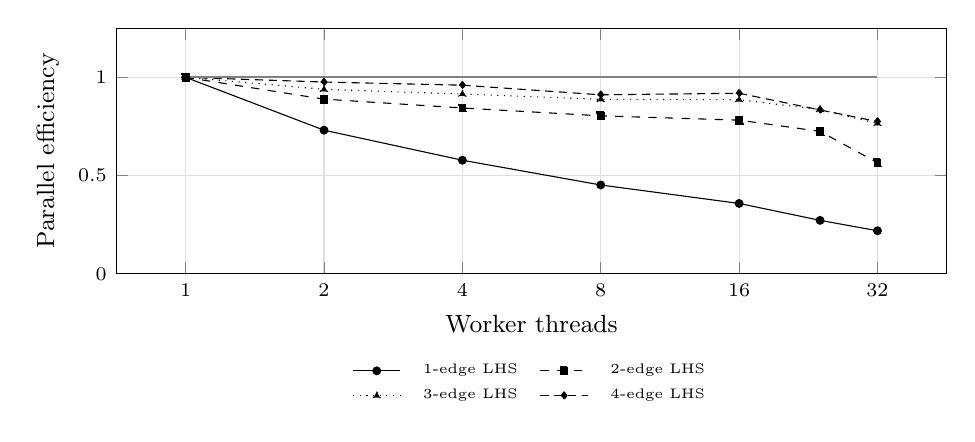
\begin{tikzpicture}
\begin{axis}[
    width=\linewidth, height=4.7cm,
    xlabel={Worker threads}, ylabel={Parallel efficiency},
    xmode=log, log basis x=2, xtick={1,2,4,8,16,32}, xticklabels={1,2,4,8,16,32},
    ymin=0, ymax=1.25, grid=major, grid style={gray!25},
    legend style={font=\tiny, at={(0.5,-0.32)}, anchor=north, legend columns=2,
                  draw=none, fill=none, column sep=6pt},
    label style={font=\small}, tick label style={font=\scriptsize},
]
% GENERATED by tools/dev/paper_tables.py -- do not edit.
% commit 61c409ca | measured on AMD EPYC 9174F 16-Core Processor | table generated on Intel(R) Core(TM) i9-14900K, 20 GB RAM, Linux 5.15.167.4-microsoft-standard-WSL2 | source: tools/dev/rich_sweep.sh over tools/sampling_cost_smoke.cpp

\addplot[mark=*, black, solid, mark size=1.4pt] coordinates {(1,1.000)(2,0.731)(4,0.578)(8,0.452)(16,0.358)(24,0.272)(32,0.219)};
\addlegendentry{1-edge LHS}
\addplot[mark=square*, black, dashed, mark size=1.4pt] coordinates {(1,1.000)(2,0.889)(4,0.844)(8,0.804)(16,0.782)(24,0.725)(32,0.565)};
\addlegendentry{2-edge LHS}
\addplot[mark=triangle*, black, dotted, mark size=1.4pt] coordinates {(1,1.000)(2,0.939)(4,0.915)(8,0.888)(16,0.886)(24,0.836)(32,0.765)};
\addlegendentry{3-edge LHS}
\addplot[mark=diamond*, black, densely dashed, mark size=1.4pt] coordinates {(1,1.000)(2,0.976)(4,0.960)(8,0.911)(16,0.919)(24,0.834)(32,0.775)};
\addlegendentry{4-edge LHS}
\addplot[gray, thick, no marks, forget plot] coordinates {(1,1)(32,1)};

\end{axis}
\end{tikzpicture}
\caption{Left-hand-side size: one to four edges, all binary chains.}
\end{subfigure}

\vspace{2mm}
\begin{subfigure}{\linewidth}
\centering
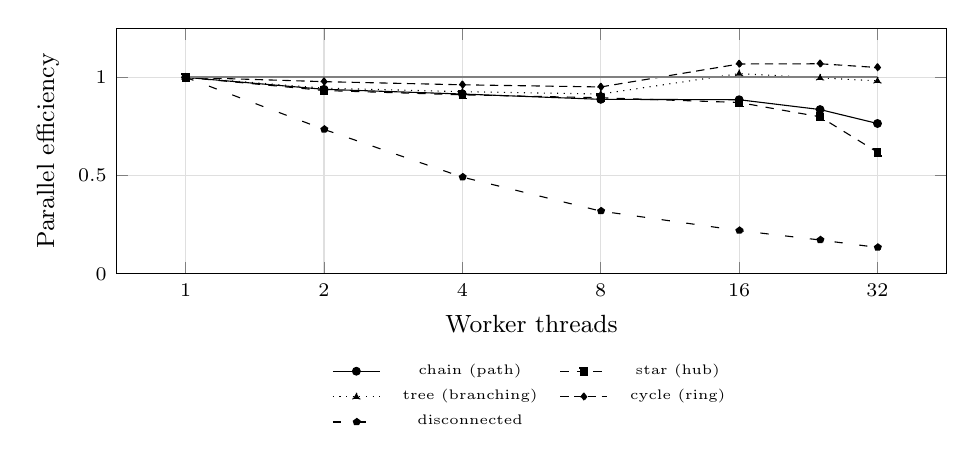
\begin{tikzpicture}
\begin{axis}[
    width=\linewidth, height=4.7cm,
    xlabel={Worker threads}, ylabel={Parallel efficiency},
    xmode=log, log basis x=2, xtick={1,2,4,8,16,32}, xticklabels={1,2,4,8,16,32},
    ymin=0, ymax=1.25, grid=major, grid style={gray!25},
    legend style={font=\tiny, at={(0.5,-0.32)}, anchor=north, legend columns=2,
                  draw=none, fill=none, column sep=6pt},
    label style={font=\small}, tick label style={font=\scriptsize},
]
% GENERATED by tools/dev/paper_tables.py -- do not edit.
% commit 61c409ca | measured on AMD EPYC 9174F 16-Core Processor | table generated on Intel(R) Core(TM) i9-14900K, 20 GB RAM, Linux 5.15.167.4-microsoft-standard-WSL2 | source: tools/dev/rich_sweep.sh over tools/sampling_cost_smoke.cpp

\addplot[mark=*, black, solid, mark size=1.4pt] coordinates {(1,1.000)(2,0.939)(4,0.915)(8,0.888)(16,0.886)(24,0.836)(32,0.765)};
\addlegendentry{chain (path)}
\addplot[mark=square*, black, dashed, mark size=1.4pt] coordinates {(1,1.000)(2,0.933)(4,0.911)(8,0.896)(16,0.872)(24,0.799)(32,0.619)};
\addlegendentry{star (hub)}
\addplot[mark=triangle*, black, dotted, mark size=1.4pt] coordinates {(1,1.000)(2,0.945)(4,0.927)(8,0.915)(16,1.019)(24,0.997)(32,0.982)};
\addlegendentry{tree (branching)}
\addplot[mark=diamond*, black, densely dashed, mark size=1.4pt] coordinates {(1,1.000)(2,0.978)(4,0.962)(8,0.951)(16,1.068)(24,1.069)(32,1.050)};
\addlegendentry{cycle (ring)}
\addplot[mark=pentagon*, black, loosely dashed, mark size=1.4pt] coordinates {(1,1.000)(2,0.735)(4,0.492)(8,0.319)(16,0.220)(24,0.172)(32,0.134)};
\addlegendentry{disconnected}
\addplot[gray, thick, no marks, forget plot] coordinates {(1,1)(32,1)};

\end{axis}
\end{tikzpicture}
\caption{Connectivity at comparable size: path, hub, branching tree, ring, two disjoint
components.}
\end{subfigure}

\vspace{2mm}
\begin{subfigure}{\linewidth}
\centering
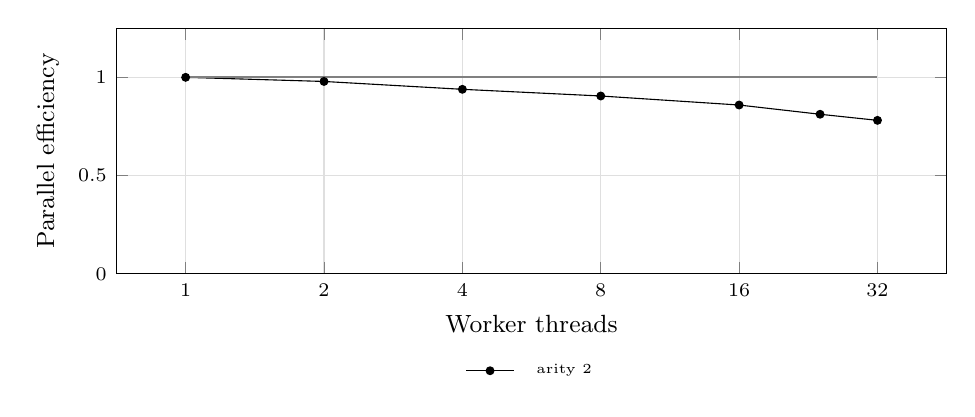
\begin{tikzpicture}
\begin{axis}[
    width=\linewidth, height=4.7cm,
    xlabel={Worker threads}, ylabel={Parallel efficiency},
    xmode=log, log basis x=2, xtick={1,2,4,8,16,32}, xticklabels={1,2,4,8,16,32},
    ymin=0, ymax=1.25, grid=major, grid style={gray!25},
    legend style={font=\tiny, at={(0.5,-0.32)}, anchor=north, legend columns=2,
                  draw=none, fill=none, column sep=6pt},
    label style={font=\small}, tick label style={font=\scriptsize},
]
% GENERATED by tools/dev/paper_tables.py -- do not edit.
% commit 97526beb | measured on AMD EPYC 9174F 16-Core Processor | table generated on Intel(R) Core(TM) i9-14900K, 20 GB RAM, Linux 5.15.167.4-microsoft-standard-WSL2 | source: tools/dev/rich_sweep.sh over tools/sampling_cost_smoke.cpp

\addplot[mark=*, black, solid, mark size=1.4pt] coordinates {(1,1.000)(2,0.979)(4,0.939)(8,0.905)(16,0.859)(24,0.812)(32,0.781)};
\addlegendentry{arity 2}
\addplot[gray, thick, no marks, forget plot] coordinates {(1,1)(32,1)};

\end{axis}
\end{tikzpicture}
\caption{Edge arity at a fixed three-edge left-hand side.}
\end{subfigure}
\caption{Parallel efficiency along the three properties of a left-hand side. Each curve is
normalized by its own single-threaded time on the same binary, workload and canonicalization
mode; the grey line $y=1$ is ideal scaling.}
\label{fig:lhs-scaling}
\end{figure}

\subsection{Evolution Depth and Relation Sizes}
\label{sec:shape-space}

Each shape is evolved one depth at a time until a single run exceeds the collection budget, so the
right-hand end of each curve in Figure~\ref{fig:shape-space} is the deepest depth that shape
reached within the budget. Runs that filled a container are excluded, because such a run returns
a truncated graph: one shape returns the same $2{,}097{,}149$ states when asked for depth 9, 10 or
11. Of the $192$ collected points, $41$ are excluded for this reason.

States and relation sizes vary independently. At around $300$k states the two-component shape has
$3.2$M branchial edges while a mixed-arity chain of similar size has none, and across the sweep the
branchial count ranges from zero to $58.8$M. Branchial edges connect pairs of events from the same
state that share a consumed edge, so their number depends on how many matches overlap rather than
on how many states exist, and a shape's position on the right panel of
Figure~\ref{fig:shape-space} is a property of its rule. Table~\ref{tab:t14-shape-space} gives the
deepest point each shape reached within the budget without filling a container, so depths differ
between rows. \texttt{chain2a3} and \texttt{chain2a4} have identical counts because in a path of
arity three or more consecutive edges already share enough vertices to fix a match's orientation,
so the two searches are the same.

A one-edge left-hand side produces no branchial edges at any depth, because two matches of a
single-edge pattern cannot share an edge. Every shape with two or more edges produces them.

\begin{figure}[htbp]
\centering
\begin{subfigure}{\linewidth}
\centering
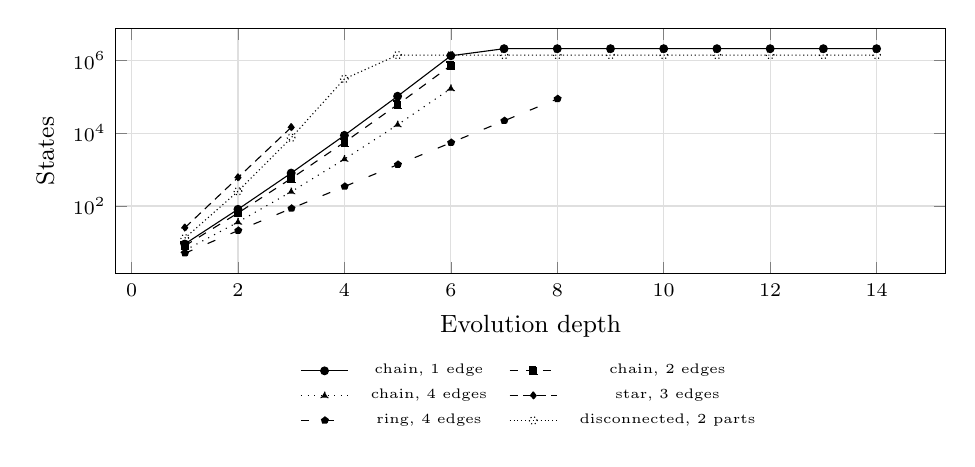
\begin{tikzpicture}
\begin{axis}[
    width=\linewidth, height=4.7cm,
    xlabel={Evolution depth}, ylabel={States},
    ymode=log, log basis y=10, grid=major, grid style={gray!25},
    legend style={font=\tiny, at={(0.5,-0.32)}, anchor=north, legend columns=2,
                  draw=none, fill=none, column sep=6pt},
    label style={font=\small}, tick label style={font=\scriptsize},
]
% GENERATED by tools/dev/paper_tables.py -- do not edit.
% commit 78c2f411 | measured on Intel(R) Core(TM) i9-14900K, 20 GB RAM, Linux 5.15.167.4-microsoft-standard-WSL2 | source: tools/dev/rich_sweep.sh over tools/sampling_cost_smoke.cpp

\addplot[mark=*, black, solid, mark size=1.4pt] coordinates {(1,9)(2,81)(3,801)(4,8721)(5,103761)(6,1339281)(7,2097148)(8,2097148)(9,2097149)(10,2097149)(11,2097149)(12,2097148)(13,2097148)(14,2097149)};
\addlegendentry{chain, 1 edge}
\addplot[mark=square*, black, dashed, mark size=1.4pt] coordinates {(1,8)(2,64)(3,568)(4,5608)(5,61048)(6,726328)};
\addlegendentry{chain, 2 edges}
\addplot[mark=triangle*, black, dotted, mark size=1.4pt] coordinates {(1,6)(2,36)(3,246)(4,1926)(5,17046)(6,168246)};
\addlegendentry{chain, 4 edges}
\addplot[mark=diamond*, black, densely dashed, mark size=1.4pt] coordinates {(1,25)(2,601)(3,14425)};
\addlegendentry{star, 3 edges}
\addplot[mark=pentagon*, black, loosely dashed, mark size=1.4pt] coordinates {(1,5)(2,21)(3,85)(4,341)(5,1365)(6,5461)(7,21845)(8,87381)};
\addlegendentry{ring, 4 edges}
\addplot[mark=o, black, densely dotted, mark size=1.4pt] coordinates {(1,13)(2,253)(3,7453)(4,309853)(5,1398101)(6,1398101)(7,1398100)(8,1398101)(9,1398101)(10,1398101)(11,1398101)(12,1398101)(13,1398101)(14,1398100)};
\addlegendentry{disconnected, 2 parts}

\end{axis}
\end{tikzpicture}
\caption{States against evolution depth, logarithmic in states.}
\end{subfigure}

\vspace{2mm}
\begin{subfigure}{\linewidth}
\centering
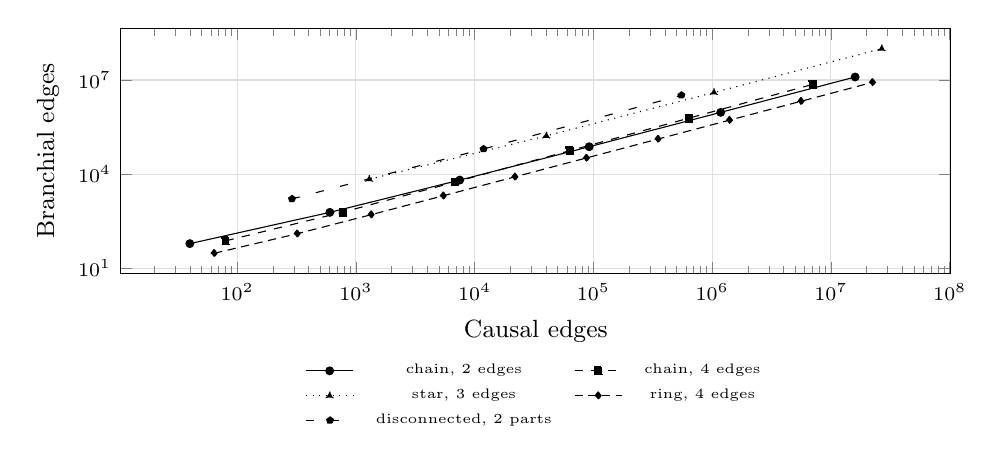
\begin{tikzpicture}
\begin{axis}[
    width=\linewidth, height=4.7cm,
    xlabel={Causal edges}, ylabel={Branchial edges},
    xmode=log, log basis x=10, ymode=log, log basis y=10,
    grid=major, grid style={gray!25},
    legend style={font=\tiny, at={(0.5,-0.32)}, anchor=north, legend columns=2,
                  draw=none, fill=none, column sep=6pt},
    label style={font=\small}, tick label style={font=\scriptsize},
]
% GENERATED by tools/dev/paper_tables.py -- do not edit.
% commit 9fb10394 | measured on AMD EPYC 9174F 16-Core Processor | table generated on Intel(R) Core(TM) i9-14900K, 31 GB RAM, Linux 5.15.167.4-microsoft-standard-WSL2 | source: tools/dev/rich_sweep.sh over tools/sampling_cost_smoke.cpp

\addplot[mark=*, black, solid, mark size=1.4pt] coordinates {(40,61)(604,606)(7492,6463)(92164,74609)(1180804,930055)(15998404,12470527)};
\addlegendentry{chain, 2 edges}
\addplot[mark=square*, black, dashed, mark size=1.4pt] coordinates {(80,75)(780,618)(6828,5588)(63276,55760)(639276,610019)(7054476,7264602)};
\addlegendentry{chain, 4 edges}
\addplot[mark=triangle*, black, dotted, mark size=1.4pt] coordinates {(1296,6900)(40176,165876)(1035504,3994260)(26779248,99436884)};
\addlegendentry{star, 3 edges}
\addplot[mark=diamond*, black, densely dashed, mark size=1.4pt] coordinates {(64,30)(320,126)(1344,510)(5440,2046)(21824,8190)(87360,32766)(349504,131070)(1398080,524286)(5592384,2097150)(22369600,8388606)};
\addlegendentry{ring, 4 edges}
\addplot[mark=pentagon*, black, loosely dashed, mark size=1.4pt] coordinates {(288,1614)(11808,62814)(547488,3238014)};
\addlegendentry{disconnected, 2 parts}

\end{axis}
\end{tikzpicture}
\caption{Branchial edges against causal edges, both logarithmic; each point is one
(shape, depth) run.}
\end{subfigure}
\caption{The state space and its relations, by left-hand-side shape.}
\label{fig:shape-space}
\end{figure}

\begin{table}[htbp]
\centering
\caption{The deepest point reached by each left-hand-side shape: \texttt{Shape}
the connectivity, \texttt{Arity} the vertices per edge, \texttt{LHS} the pattern's edge count;
the remaining columns are the sizes of the three objects the run built.}
\label{tab:t14-shape-space}
% GENERATED by tools/dev/paper_tables.py -- do not edit.
% commit 97526beb | measured on AMD EPYC 9174F 16-Core Processor | table generated on Intel(R) Core(TM) i9-14900K, 20 GB RAM, Linux 5.15.167.4-microsoft-standard-WSL2 | source: tools/dev/rich_sweep.sh over tools/sampling_cost_smoke.cpp
{\footnotesize\setlength{\tabcolsep}{4pt}%
\resizebox{\ifdim\width>\linewidth\linewidth\else\width\fi}{!}{%
\begin{tabular}{lrrrrrrr}
\toprule
Rule & Shape & Arity & LHS & Depth & States & Causal & Branchial \\
\midrule
\texttt{chain1a2} & chain & 2 & 1 & 6 & 1,339,281 & 850,896 & 0 \\
\texttt{growth} & chain & 2 & 1 & 10 & 4,037,914 & 4,037,912 & 0 \\
\texttt{chain2a2} & chain & 2 & 2 & 5 & 61,048 & 92,164 & 74,609 \\
\texttt{pair} & chain & 2 & 2 & 7 & 204,556 & 393,788 & 181,439 \\
\texttt{chain2a3} & chain & 3 & 2 & 5 & 19,608 & 26,732 & 16,806 \\
\texttt{chain2a4} & chain & 4 & 2 & 5 & 19,608 & 26,732 & 16,806 \\
\texttt{chain3a2} & chain & 2 & 3 & 5 & 33,649 & 87,920 & 81,725 \\
\texttt{triple} & chain & 2 & 3 & 6 & 23,116 & 66,980 & 37,362 \\
\texttt{chain3a3} & chain & 3 & 3 & 5 & 9,331 & 23,612 & 13,995 \\
\texttt{chain4a2} & chain & 2 & 4 & 5 & 17,046 & 63,276 & 55,760 \\
\texttt{quad} & chain & 2 & 4 & 6 & 23,116 & 90,092 & 51,609 \\
\texttt{cycle3a2} & cycle & 2 & 3 & 9 & 29,524 & 88,560 & 29,523 \\
\texttt{cycle4a2} & cycle & 2 & 4 & 7 & 21,845 & 87,360 & 32,766 \\
\texttt{disc2a2} & disc & 2 & 2 & 4 & 309,853 & 547,488 & 3,238,014 \\
\texttt{disc} & disc & 2 & 2 & 4 & 309,853 & 547,488 & 3,238,014 \\
\texttt{disc3a2} & disc & 2 & 3 & 4 & 1,045,591 & 3,136,752 & 58,835,751 \\
\texttt{mixed2} & mixed & 2 & 2 & 8 & 87,381 & 148,520 & 0 \\
\texttt{mixed3} & mixed & 2 & 3 & 9 & 29,524 & 85,978 & 19,682 \\
\texttt{mixed4} & mixed & 2 & 4 & 9 & 29,524 & 115,976 & 19,682 \\
\texttt{star2a2} & star & 2 & 2 & 4 & 26,293 & 45,792 & 108,378 \\
\texttt{star3a2} & star & 2 & 3 & 3 & 14,425 & 40,176 & 165,876 \\
\texttt{star4a2} & star & 2 & 4 & 3 & 14,425 & 57,600 & 165,876 \\
\texttt{tree3a2} & tree & 2 & 3 & 5 & 34,599 & 89,552 & 82,480 \\
\texttt{tree4a2} & tree & 2 & 4 & 5 & 40,655 & 148,628 & 179,283 \\
\bottomrule
\end{tabular}
}}

\end{table}

\subsection{Memory Behavior under Thread Scaling}
\label{sec:memory-scaling}
Falling efficiency at high thread counts could come from contention on the shared structures or
from the cost of acquiring memory. Table~\ref{tab:t13-memory} gives \texttt{getrusage} figures for
a workload of eighteen seconds of single-threaded work. Across a $\ThreadSweepFactor\times$
increase in workers, user time grows $\UserTimeGrowth\times$ and system time
$\SysTimeGrowth\times$, reaching $2.9$\,s of $128.7$\,s of CPU time at 32 workers, so the extra
time is in user code. Peak
resident set grows by a quarter and minor faults eleven-fold, and system time, which follows the
faults as each worker draws its own arena blocks, stays small, so memory acquisition is not the
cause. The instruction count is flat across the sweep (below), so spinning is not the cause either.

Hardware counters identify the cause. On the Wolfram rule at depth seven, executed instructions
are $14.5$G at one thread and $15.8$G at 32, while cycles double, so instructions per cycle fall
from $1.44$ to $0.69$. The counter that grows is demand fills served from another L3 domain's cache
(AMD \texttt{ls\_dmnd\_fills\_from\_sys.near\_cache}): $47$k at one thread and $10.6$M at 32. Fills
from DRAM and from the local cache hierarchy stay flat. Two experiments rule out the concurrent
structures as the source. Limiting the shared table's probe length from $32$ to $4$ leaves the fill
count unchanged and makes the run slower. A thread-private filter that removes $80\%$ of the
repeated inserts into the shared set lowers the set's share of the fills from $36\%$ to $12\%$
without changing the total or the wall time; the fills move to neighboring code. The traffic comes
from the evolution itself: about twelve cross-domain fills per object created, because a state
created on one core complex is read by workers on others, and this part has eight L3 domains.

The effect is visible in wall time when a run first uses a second L3 domain. Sweeping every worker
count from one to thirty-two, with workers pinned one per physical core in order, on a part whose
L3 domains hold two cores each: wall time falls from one worker to two, rises from two to three
on every large workload (\texttt{wpp} by $12.7\%$, \texttt{wolfram24} by $20.4\%$,
\texttt{wolftri} by $12.8\%$, \texttt{multirule} by $36.1\%$), and falls again from four onward.
The third worker is the first in a second domain. Placing that worker on an SMT sibling in the
first domain removes the rise (\texttt{wpp} $347$ to $258$\,ms at three workers, below the
two-worker time), and the rise moves to the fourth worker, which opens the second domain. Filling
each domain's two cores and their two SMT siblings before using the next domain is faster at every
count measured, including sixteen workers (\texttt{wpp} $197$ to $182$\,ms, \texttt{wolfram24}
$36.3$ to $33.3$\,ms, \texttt{multirule} $34.7$ to $25.7$\,ms), although it uses half as many
physical cores at sixteen. This packed placement is the engine's default and was used for every
table in this section. Under it the rise moves to the fifth worker, the first in a second domain:
\texttt{wpp} takes $216$\,ms at four workers, $247$ at five, $234$ at six and $205$ at eight, and
later domains add at most $2.3\%$ at any count from one to thirty-two. At powers of two the curve
falls monotonically. These measurements depend on the host: on a part with larger L3 domains the
second domain opens at a higher worker count.

\begin{table}[htbp]
\centering
\caption{User and system time, peak resident set and minor page faults against
thread count, from \texttt{getrusage}.}
\label{tab:t13-memory}
% GENERATED by tools/dev/paper_tables.py -- do not edit.
% commit f53a191 | measured on AMD EPYC 9174F 16-Core Processor, 503 GB RAM, Linux 6.8.0-138-generic | load at start 3.10/1.73 (1m/15m) | source: tools/sampling_cost_smoke.cpp under procstat.measure
{\footnotesize\setlength{\tabcolsep}{4pt}%
\resizebox{\ifdim\width>\linewidth\linewidth\else\width\fi}{!}{%
\begin{tabular}{rrrrrr}
\toprule
Threads & Wall s & User s & System s & Peak RSS MB & Minor faults \\
\midrule
1 & 3.09 & 2.73 & 0.35 & 624 & 160\,040 \\
8 & 1.00 & 6.36 & 0.80 & 1184 & 311\,547 \\
16 & 0.80 & 8.46 & 1.51 & 1816 & 483\,330 \\
24 & 0.77 & 10.60 & 2.39 & 2377 & 633\,698 \\
32 & 0.82 & 12.73 & 3.25 & 2865 & 768\,659 \\
\bottomrule
\end{tabular}
}}

\end{table}

\subsection{Device Saturation}
The resident kernel is launched with a fixed number of blocks per streaming multiprocessor, so that
number is a tuning parameter. Wall time falls as blocks are added until eight per SM, the default,
and sixteen per SM is within measurement variation of eight (Table~\ref{tab:t11-saturation}). The
last column, the driver's peak SM-busy reading, reports whether the multiprocessors were busy, not
how many warps were resident; it reads $100\%$ at every point.

\begin{table}[htbp]
\centering
\caption{Wall time and peak SM-busy against blocks per streaming multiprocessor.}
\label{tab:t11-saturation}
% GENERATED by tools/dev/paper_tables.py -- do not edit.
% commit 769b12ba | Intel(R) Core(TM) i9-14900K, 20 GB RAM, Linux 5.15.167.4-microsoft-standard-WSL2 | source: tools/bench_gpu_evolve.cpp (mode 2) + driver utilisation sampling
\resizebox{\ifdim\width>\linewidth\linewidth\else\width\fi}{!}{%
\begin{tabular}{rrrrl}
\toprule
Blocks per SM & Blocks & Median ms & vs.\ 1 per SM & Peak SM-busy \\
\midrule
1 & 128 & 6.15 & 1.00$\times$ & 91\% \\
2 & 256 & 6.13 & 1.00$\times$ & 92\% \\
4 & 512 & 5.40 & 1.14$\times$ & 98\% \\
8 & 1024 & 5.91 & 1.04$\times$ & 86\% \\
16 & 2048 & 5.75 & 1.07$\times$ & 97\% \\
\bottomrule
\end{tabular}
}

\end{table}

\subsection{Occupancy and Lane Efficiency}
\label{sec:device-bounds}

Table~\ref{tab:device-occupancy} gives occupancy, throughput and active lanes per warp for the
resident kernel on every corpus workload, from hardware counters under Nsight Compute.

\textbf{Occupancy.} \texttt{cuobjdump -res-usage} on the linked binary reports that
\texttt{k\_persistent\_evolve} uses 255 registers per thread, the architectural maximum. At 32
threads per block a block reserves $8{,}160$ registers, and an sm\_89 multiprocessor has
$65{,}536$, so eight blocks fit: 256 resident threads against a maximum of $1{,}536$, an occupancy
of $16.7\%$. The launch grid is also eight blocks per multiprocessor, so the two limits coincide.
The measured occupancy is $14.1\%$ to $17.3\%$ on every corpus workload, over kernel durations that
differ by a factor of seven hundred. Limiting the kernel to 128 registers halves the register
allocation and leaves occupancy unchanged, so the grid, not the register count, sets it. Doubling
the grid under that limit doubles residency and makes the kernel slower, increasingly so as the grid
grows, because the added warps compete for the shared work queues without adding independent work.

\textbf{Active lanes.} The canonicalization phase runs on the whole warp: refinement's loops are
spread across the lanes, and the search's serial steps (individualization, orbit closure, backtracking)
run on one lane while the others wait at warp barriers. Publication, signature, quotient and
deduplication steps run on one lane. On \texttt{wpp} at depth six the kernel averages $3.5$ active
lanes per warp out of $32$. Per-block \texttt{clock64} timing shows that, on the workloads with
enough work to measure, canonicalization takes most block cycles, rewriting a few percent and
matching under two.

\textbf{Throughput.} No hardware unit is near its limit. On \texttt{wpp} at depth six SM
throughput is $9.7\%$ of peak, memory throughput $24.3\%$ and DRAM $11.6\%$; across the corpus the
maxima are $12.6\%$, $33.8\%$ and $16.1\%$. Atomic operations, which the work queues use, are
served by L2, whose throughput is included in the memory figure.

On the large workloads the device is therefore limited by the serial steps of the IR search, in
which each step depends on the one before, and not by bandwidth, queue contention or occupancy. A
separate measurement records no time spent waiting for unpublished work.

\textbf{Workloads with few classes.} The workloads with few states behave differently. With causal
recording on, \texttt{cycle4} and \texttt{multirule} reconstruct causal relations far larger than
their state counts and still leave the device idle most of the time, with SM throughput of $2.2\%$
and DRAM $0.01\%$ on \texttt{cycle4}, and $9.8$ and $10.4$ active lanes. The kernel takes four
times longer on \texttt{multirule}'s $49$ states than on \texttt{wolfram24}'s $9{,}820$. At depth
six \texttt{cycle4} replays $68{,}185$ instances over $40$ classes and is slower than the host,
while \texttt{wolfram24} replays $86{,}086$ instances over $9{,}820$ classes and is faster. The
instance counts are similar and the class counts differ by a factor of 250. The replay walks each
class's instances on one worker, so a run with forty classes has forty workers' worth of parallel
work however many instances it holds. \texttt{cycle4} starts from an initial state with many
automorphisms, which collapses its states into few classes.

\textbf{Causal recording.} The measurements above run with causal recording off. With it on, the
device and host reconstruct the same causal relation on all eight corpus workloads the device
supports, at depth six: the same number of distinct pairs and the same number after transitive
reduction. On the densest available workload, a three-edge disconnected left-hand side at depth
three, both give $1{,}661{,}760$ causal pairs and $970{,}560$ after reduction. The two engines
share only the replay core, with separate schedulers, memory layouts and queues. Both store the
relation unreduced and reduce it when it is read, using one shared reduction; a finite DAG has one
transitive reduction, so the result does not depend on the order in which pairs arrive. The
reduction is computed once per source event, since every edge leaving an event shares the set
reachable from it in two or more steps, and when event identifiers increase along every causal
edge the search stops at the source's largest target. Branchial pairs are not stored: both engines
derive them from the applications when they are read.

\textbf{Host traffic.} Across every evolution traced, no copy, allocation or memset runs while the
resident kernel runs, including twenty-four consecutive evolutions with the reconstruction on. Each
evolution is preceded and followed by runtime allocation, copy and fill calls, in equal numbers, so
a session pays this cost on every call, and a single deep run pays it once.

When raw events are not requested, the replay does not run (Section~\ref{sec:quotient}). With the
replay on, \texttt{multirule} and \texttt{cycle4} do not complete depth seven; without it both
complete, with the same state and event counts.

\begin{table}[htbp]
\centering
\caption{\textbf{Resident-kernel occupancy, throughput and active lanes across the corpus},
from hardware counters under NVIDIA Nsight Compute: means over the profiled launches of the
resident kernel. Durations are the profiler's, which serializes execution and fixes clocks, and
are not comparable with the wall times of Table~\ref{tab:t7b-gpu-corpus}.}
\label{tab:device-occupancy}
\resizebox{\ifdim\width>\linewidth\linewidth\else\width\fi}{!}{%
% GENERATED by tools/dev/paper_tables.py -- do not edit.
% commit e264560a | measured on AMD EPYC 9174F 16-Core Processor, NVIDIA GeForce RTX 4090 | table generated on Intel(R) Core(TM) i9-14900K, 31 GB RAM, Linux 5.15.167.4-microsoft-standard-WSL2 | source: Nsight Compute over tools/bench_gpu_evolve.cpp (mode 2)
{\footnotesize\setlength{\tabcolsep}{4pt}%
\resizebox{\ifdim\width>\linewidth\linewidth\else\width\fi}{!}{%
\begin{tabular}{lrrrrrrrr}
\toprule
Workload & Depth & Launches & Duration (\textmu s) & SM \% & Mem.\ \% & DRAM \% & Lanes/warp & Occ.\ \% \\
\midrule
\texttt{disc2x2} & 6 & 7 & 178994.3 & 3.88 & 3.95 & 0.17 & 6.05 & 16.84 \\
\texttt{multirule} & 6 & 5 & 113454.0 & 2.24 & 2.30 & 0.02 & 10.41 & 17.25 \\
\texttt{growshrink3} & 6 & 12 & 81015.0 & 10.86 & 33.27 & 16.08 & 3.14 & 16.99 \\
\texttt{cycle4} & 6 & 3 & 73393.3 & 2.23 & 2.72 & 0.01 & 9.84 & 16.39 \\
\texttt{multiroot} & 6 & 3 & 13420.0 & 2.38 & 2.43 & 0.04 & 8.87 & 15.54 \\
\texttt{wolfram24} & 6 & 3 & 9086.7 & 12.59 & 33.75 & 12.88 & 2.71 & 16.41 \\
\texttt{wpp} & 6 & 3 & 3900.0 & 9.65 & 24.25 & 11.57 & 3.45 & 16.71 \\
\texttt{binary} & 6 & 3 & 2676.7 & 2.20 & 2.22 & 0.03 & 11.17 & 16.77 \\
\texttt{arity3} & 6 & 3 & 2106.7 & 2.20 & 2.17 & 0.03 & 11.59 & 16.42 \\
\texttt{triangle} & 6 & 3 & 263.8 & 2.60 & 2.95 & 0.21 & 11.59 & 16.28 \\
\bottomrule
\end{tabular}
}}
}
\end{table}

\subsection{Ablation}
Match forwarding is the one run-time switch that changes speed without changing the answer. The
state and event identity modes change which answer is computed, so a time ratio between them
compares different computations; Section~\ref{sec:event-canon} reports how their results differ,
and Table~\ref{tab:t6-quotient} reports quotient exploration. The static analysis of
Section~\ref{sec:static-analysis} turns forwarding on or off per rule set. Table~\ref{tab:t9-ablation}
gives best-of-$N$ wall times for both settings. On the one-edge left-hand side (depth eight) the
analysis turns forwarding off, and forwarding on is $1.16\times$ slower. On the two-edge left-hand
side (depth six) it turns forwarding on, and forwarding on is $1.10\times$ slower than off, a
difference within the run-to-run variation of runs that short on this machine. Both settings give
the same state and event counts on both workloads.

\begin{table}[htbp]
\centering
\caption{Match forwarding on and off: one-edge left-hand side at depth eight, two-edge at depth
six. Best-of-$N$ wall times; both settings give identical state and event counts.}
\label{tab:t9-ablation}
% GENERATED by tools/dev/paper_tables.py -- do not edit.
% commit e0cdb45f | Intel(R) Core(TM) i9-14900K, 20 GB RAM, Linux 5.15.167.4-microsoft-standard-WSL2 | source: tools/sampling_cost_smoke.cpp
\resizebox{\ifdim\width>\linewidth\linewidth\else\width\fi}{!}{%
\begin{tabular}{lllrlrl}
\toprule
Contribution & Arm A & A ms & Arm B & B ms & Ratio & Same answer \\
\midrule
Match forwarding, one-edge LHS & on & 116.9 & decided off & 94.5 & 1.24 & yes \\
Match forwarding, two-edge LHS & off & 239.9 & decided on & 157.9 & 1.52 & yes \\
State canonicalization & Full (exact) & 158.4 & Automatic (hash) & 168.8 & 0.94 & yes \\
\bottomrule
\end{tabular}
}

\end{table}

\subsection{Instruction Profile}
\label{sec:instruction-profile}

Executed instruction counts are deterministic for a single-threaded run and unaffected by other
load, so they attribute time to parts of the engine. Table~\ref{tab:t15-instructions}
comes from one \texttt{callgrind} run of a single-threaded depth-six evolution of the Wolfram rule
under quotient exploration with the raw relations reconstructed, the CPU benchmark's default
configuration. The quotient reconstruction ($\InstrShareRecon\%$) and canonicalization
($\InstrShareCanon\%$) are the two largest parts and are close; the concurrent sets and maps
($\InstrShareSets\%$) and libc's copies, fills and heap calls ($\InstrShareLibc\%$) follow; matching,
its join and the rewrite together are $\InstrShareMatch\%$. The unattributed $\InstrUnattributedPct\%$
is functions below the reporting threshold and code not assigned to a group.

\begin{table}[htbp]
\centering
\caption{Executed instructions by component: a single-threaded depth-six
evolution of the Wolfram rule under quotient exploration with reconstruction, under
\texttt{callgrind}, grouped by the algorithm each function belongs to. The per-function profile
covers $\InstrFlatCoverage\%$ of the program total; the rest is below the annotator's reporting
threshold. The benchmark-harness row is the corpus set-up the benchmark performs before the
evolution.}
\label{tab:t15-instructions}
% GENERATED by tools/dev/paper_tables.py -- do not edit.
% commit 61c409ca | measured on AMD EPYC 9174F 16-Core Processor | table generated on Intel(R) Core(TM) i9-14900K, 20 GB RAM, Linux 5.15.167.4-microsoft-standard-WSL2 | source: tools/dev/remote_session.sh attrib phase, callgrind over tools/bench_cpu_evolve
{\footnotesize\setlength{\tabcolsep}{4pt}%
\resizebox{\ifdim\width>\linewidth\linewidth\else\width\fi}{!}{%
\begin{tabular}{lrr}
\toprule
Component & Instructions & Share \\
\midrule
Match expansion and join & 117,653,606 & 24.7\% \\
Canonicalization (IR) & 79,592,324 & 16.7\% \\
Dedup sets and maps & 71,807,564 & 15.1\% \\
Arena allocation & 38,097,485 & 8.0\% \\
Hypergraph storage & 24,250,782 & 5.1\% \\
Causal and branchial & 728,120 & 0.2\% \\
Job system and work stealing & 366,201 & 0.1\% \\
\midrule
Unattributed & 139,143,506 & 29.2\% \\
\midrule
\textbf{Total} & 476,371,312 & 99.0\% \\
\bottomrule
\end{tabular}
}}

\end{table}

\paragraph{Cost per unit of work.} Each phase's instruction count divided by the number of items it
produces, from the same run: $\InstrIrCalls$ canonicalization calls over $\InstrRaw$ raw states,
$\InstrEvents$ reconstructed events, $\InstrSetInserts$ claim-set inserts and $\InstrCaptured$
applied matches. Canonicalization costs $\InstrIrPerCanonCall$ instructions per call on states of
two to fourteen edges. The search goes past its first node on $\InstrIrSearched$ of the
$\InstrIrCalls$ calls, so most calls cost one refinement to a stable partition, a few thousand
instructions at this size; the measured cost is several times that, with $\InstrCanonRefinePct\%$
of the phase in the refinement loop, $\InstrCanonHashPct\%$ in per-call set-up and the invariant
hash, and $\InstrCanonOrbitsPct\%$ in the orbit computation that quotient event identity needs.
Reconstruction costs $\InstrIrPerReconEvent$ instructions per event, against a minimum of one
identity claim, one producer lookup per consumed edge and one producer record per produced edge, a
few hundred instructions for a rule with two inputs and four outputs; the rest is in the
per-instance replay (\texttt{qr\_apply}) and in \texttt{register\_quotient\_transition}'s vector
operations. The claim sets cost $\InstrIrPerSetInsert$ instructions per insert against a minimum of
one hash, one probe and one exchange, about fifty; $\InstrSetRepeatPct\%$ of inserts offer a key
already present. Matching, the join and the rewrite cost $\InstrIrPerAppliedMatch$ instructions per
applied match, including building the match record and the child state. Every host phase costs more
than twice its minimum. The libc share is mostly the benchmark's own set-up, inlined into
\texttt{main} by link-time optimization, and the construction of rule objects.

\subsection{Event Identity}
Table~\ref{tab:event-canon} evolves each workload once, single-threaded in the exact state mode,
and counts distinct events under each of the three conventions of Section~\ref{sec:event-canon}:
by endpoint states, by consumed and produced edges, and by distinct applications. Each convention
refines the one before, so the counts do not decrease from left to right, and they differ on most
workloads: on \texttt{binary-growth} they are $5$, $8$ and $9$. Every other event count in this
paper counts distinct applications.

\begin{table}[htbp]
\centering
\caption{Distinct events per identity convention on each corpus workload.}
\label{tab:event-canon}
% GENERATED by tools/dev/paper_tables.py -- do not edit.
% commit eb8a742 | measured on AMD EPYC 9174F 16-Core Processor, 503 GB RAM, Linux 6.8.0-138-generic | load at start 1.04/1.78 (1m/15m) | source: tools/mode_matrix_probe.cpp
{\footnotesize\setlength{\tabcolsep}{4pt}%
\resizebox{\ifdim\width>\linewidth\linewidth\else\width\fi}{!}{%
\begin{tabular}{lrrrrr}
\toprule
Workload & Steps & Canon.\ states & By endpoint states & By consumed/produced edges & Distinct applications \\
\midrule
binary-growth & 3 & 6 & 5 & 8 & 9 \\
wolfram-2to4 & 2 & 4 & 3 & 4 & 6 \\
triangle & 2 & 3 & 2 & 4 & 4 \\
reductive-2to1 & 3 & 4 & 3 & 6 & 15 \\
idempotent-2to2 & 3 & 1 & 1 & 1 & 3 \\
self-loop & 3 & 2 & 1 & 1 & 1 \\
mixed-arity & 3 & 4 & 3 & 3 & 3 \\
arity3-growth & 3 & 9 & 9 & 9 & 9 \\
disconnected-lhs & 3 & 1 & 1 & 4 & 14 \\
arity4-growth & 3 & 9 & 9 & 9 & 9 \\
mixed-arity-lhs & 3 & 2 & 1 & 1 & 1 \\
mixed-arity-init & 3 & 4 & 4 & 4 & 4 \\
arity3-to-2 & 3 & 4 & 4 & 4 & 4 \\
arity1-with-binary & 3 & 2 & 1 & 1 & 1 \\
cycle4-automorphic & 3 & 4 & 3 & 15 & 144 \\
star4-automorphic & 2 & 5 & 4 & 12 & 24 \\
multi-rule & 2 & 10 & 11 & 11 & 11 \\
\bottomrule
\end{tabular}
}}

\end{table}

\subsection{Limitations}
\label{sec:limitations}

\textbf{Two machines.} The Wolfram comparison ran on an Intel i9-14900K desktop and everything else
on the AMD EPYC host of Section~\ref{sec:benchmarks}. The scaling results depend on that host's
memory system and core count, and the thread count at which efficiency declines differs on other
hardware.

\textbf{Quotient reconstruction grows with the raw system.} Quotient exploration visits one state
per isomorphism class, but the reconstruction of raw observables creates as many instances as the
raw system has. On a two-rule set whose canonical state count grows linearly with depth (three to
eight states at depths two to seven), the reconstruction took 0.17, 0.22, 0.62, 7.36, 144.78 and
4981.05 milliseconds, about twentyfold per step. Runs that request only canonical states skip it.

\textbf{The reconstruction does not scale with threads.} Every worker takes part in the
reconstruction, and its total cycle count grows with the thread count: 511 million cycles on one
thread and 3.85 billion on thirty-two for the same work, on the densest reconstruction workload in
the corpus. The deduplication marks prevent duplicate results but not duplicate traversal. On that
workload wall time improves up to eight threads and gets worse beyond; the corpus workloads with
small reconstructions do not show the effect.

\textbf{Two comparison points, one of them our own.} The engine is compared with the
\texttt{Wolfram/\allowbreak Multicomputation} paclet's \texttt{MultiwaySystem} and with this
project's reference implementation. \texttt{MultiwaySystem} is the only other implementation we
know of that computes the deduplicated states graph under isomorphism; SetReplace computes a
different object (Section~\ref{sec:background}). The reference implementation was written by the
same author as the engine, from the same definition.

\textbf{Workload scope.} The oracle corpus has 17 workloads (Tables~\ref{tab:t1-exactness},
\ref{tab:t3-deheap} and~\ref{tab:event-canon}), and the left-hand-side sweep of
Section~\ref{sec:lhs-space} has 24 shapes (Table~\ref{tab:t14-shape-space}). Both were built to
cover rule shapes (productive, reductive, idempotent, mixed arity, disconnected and highly
symmetric), not sampled from rules used in practice, and the observed $C/R$ and parallel efficiency
describe those shapes.

\textbf{Scope of the concurrency results.} The model-checked properties hold for the stated thread
and operation counts, which are small, and the determinism gate covers the configurations it runs.

\textbf{Worst-case cost.} IR is exponential in the worst case and runs on every state in the exact
mode. States with large automorphism groups are where that cost occurs, and
Proposition~\ref{prop:wlceiling} bounds how much a cheaper pre-filter can save.

% ----------------------------------------------------------------------------
% CONCLUSION
% ----------------------------------------------------------------------------
